\documentclass[polish, 11pt, a4paper]{article}

\usepackage{polski}
\usepackage[utf8]{inputenc}
\usepackage[autostyle]{csquotes}
\DeclareQuoteAlias{dutch}{polish}
\usepackage[T1]{fontenc}
\usepackage{geometry}
\geometry{
	a4paper,
	total={170mm,257mm},
	left=25mm,
	right=25mm,
	top=20mm,
}

\usepackage{babel}
\usepackage{microtype}
\usepackage{lmodern}
\usepackage{multirow}
\usepackage{amsmath}
\usepackage{caption}
\usepackage{graphicx}
\usepackage{graphics}
\usepackage{float}
\usepackage{enumitem}
\usepackage{ragged2e}
\usepackage{parskip}
\RaggedRightParindent = 24 pt
\usepackage{indentfirst}

\begin{document}
	\begin{titlepage}
	\centering
	\Huge Laboratorium Podstaw Fizyki\\
	\vspace{1cm}
	\huge Ćwiczenie 8 \enquote{Wyznaczanie współczynnika lepkości cieczy na podstawie prawa Stokesa}\\
	\vspace{1cm}
	\raggedright
	\huge Prowadzący: mgr Karolina Paradowska\\
	\vspace{.5cm}
	\begin{table}[h]
		\centering
		\resizebox{\columnwidth}{!}{%
		\begin{tabular}{|r|l|}\hline
			Imię i Nazwisko	&Marcin Kotas\\\hline
			Nr indeksu		&235098\\\hline
			Wydział			&Elektroniki\\\hline
			Termin zajęć	&24.10.2017, godz. 9.15\\\hline
			Numer grupy ćwiczeniowej&5\\\hline
			Data oddania sprawozdania&31.10.2017\\\hline
		\end{tabular}%
		}
	\end{table}
	\end{titlepage}
	\section{Wstęp teoretyczny}
		\RaggedRight
		Celem ćwiczenia było wyznaczenie współczynnika lepkości cieczy na podstawie prawa Stokesa. Prawo Stokesa, odkryte w 1851 przez George'a Stokesa, określa siłę oporu działającą na sferyczny przedmiot poruszający się w płynie. Wzór, który posłuży do wyznaczenia współczynnika lepkości to:
		\begin{displaymath}
		\eta=\frac{d^2\cdot g\cdot t(\rho_k-\rho_c)}{18h}
		\end{displaymath}
		
		Aby uzyskać dane potrzebne do wyznaczenia współczynnika lepkości posłużyliśmy się szklanym cylindrem wypełnionym roztworem gliceryny. Wkładaliśmy do niego po kolei 3 kulki wykonane z różnych materiałów, za każdym razem mierząc czas opadania kulki między zaznaczonymi pierścieniami na cylindrze. Czas tonięcia każdej kulki oraz jej średnica zostały zmierzone 10 razy. Dodatkowo została zmierzona raz masa każdej kulki, odległość między pierścieniami na cylindrze oraz gęstość cieczy.
		\begin{figure}[h]
			\centering
			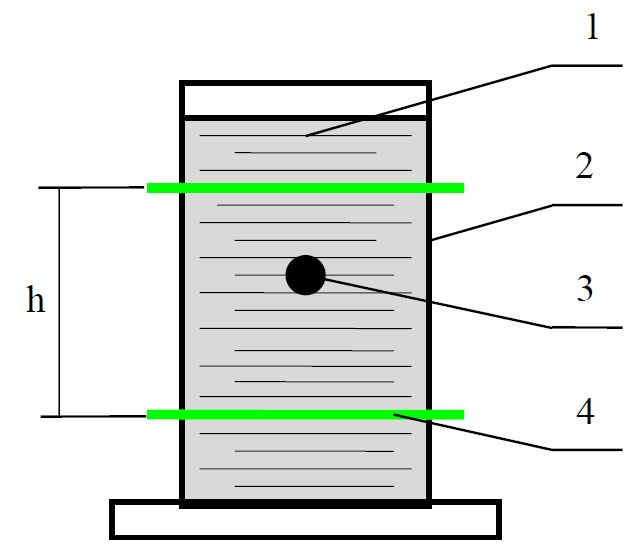
\includegraphics[width=.5\linewidth]{Fiz8Rys}
			\caption{Zestaw pomiarowy}
			\vspace{.25cm}
			1 - roztwór gliceryny, 2 - szklany cylinder, 3 - kulka,\\
			4 - pierścienie, h - dystans między pierścieniami
		\end{figure}
	\section{Wyniki pomiarów}
		
	\subsection{Wykonanie pomiarów}
		Aby zmierzyć współczynnik lepkości cieczy wykonane zostały pomiary czasu spadania w tej cieczy trzech kulek wykonanych z różnych materiałów. Czas tonięcia każdej kulki oraz jej średnica zostały zmierzone 10 razy. Dodatkowo została zmierzona raz masa każdej kulki, odległość między pierścieniami na cylindrze oraz gęstość cieczy. Wszystkie wyniki zostały przedstawione w Tabelach 1-3.
	\subsection{Obliczenia}
	\subsubsection{Opracowanie wyników}
		Najpierw wyliczono wartości średnie średnic kulek oraz czasów spadania w cieczy. Przykładowo, średni czas spadania kulki białej:
		\begin{displaymath}
		\bar{t}=\frac{1}{10}\sum_{i=1}^{10}t_i=\frac{1}{10}(20,34+21,18+\dots+20,41+20,10)=\frac{1}{10}\cdot 206,37\approx 20,64[s]
		\end{displaymath}
		Następnie wyliczona została niepewność typu A dla wszystkich średnic oraz czasów spadania. Dla czasu spadania kulki białej:
		\begin{align*}
		u_A(t)&=\sqrt{\frac{\sum_{i=1}^{10} (t_i-\bar{t})^2}{10(10-1)}}\\
				&=\sqrt{\frac{(20,34-20,64)^2+(21,18-20,64)^2+\dots+(20,10-20,64)^2}{90}}\\
				&=0,11741711\approx 0,1174[s]
		\end{align*}
		Niepewność typu B jest różna dla średnic kulek i czasów spadania, ponieważ w niepewności czasu spadania należy uwzględnić niepewność eksperymentatora (przyjęto \(\Delta{_et}=0,2[s]\)).\\
		Dla średnicy kulki białej niepewność typu B jest równa:
		\begin{displaymath}
		u_B(d)	= \frac{\Delta{_pd}}{\sqrt{3}}=\frac{0,01}{\sqrt{3}}\approx 0,005774[mm]
		\end{displaymath}
		Niepewność typu B czasu spadania:
		\begin{displaymath}
		u_B(t)	=\sqrt{\frac{(\Delta{_pt})^2}{3}+\frac{(\Delta{_et})^2}{3}}=\sqrt{\frac{0,01^2}{3}+\frac{0,2^2}{3}}
				=0,115614301\approx 0,1156[s]
		\end{displaymath}
		Finalna niepewność standardowa całkowita wynosi:
		\begin{displaymath}
			u(t)=\sqrt{u_A^2(t)+u_B^2(t)}=\sqrt{0,1174^2+0,1156^2}=0,164783022\approx 0,17[s]
		\end{displaymath} 
		Niepewność standardowa całkowita pomiarów masy kulek, odległości między pierścieniami oraz gęstości cieczy jest równa niepewności standardowej typu B. Masa została zmierzona miernikiem elektronicznym więc jej niepewność zostaje zaokrąglona do rozdzielczości miernika:
		\begin{align*}
		u(m)		&=u_b(m)=\frac{0,01}{\sqrt{3}} = 0,005774 \approx 0,01[g]\\
		u(h)		&=u_b(h)=\frac{0,1}{\sqrt{3}} = 0,05774 \approx 0,058[cm]\\
		u(\rho_c)	&=u_b(\rho_c)=\frac{10}{\sqrt{3}}= 5,774\approx 5,8 \left[\frac{kg}{m^3}\right]
		\end{align*}
		Na podstawie wyników wyliczona została gęstość każdej kulki. Gęstość kulki białej wynosi:
		\begin{displaymath}
		\rho_k	=\frac{6 m}{\pi \cdot d^3}=\frac{6\cdot 0,44\cdot 10^{-3}}{\pi \cdot (7,9010\cdot 10^{-3})^3}
			=1703,757846\approx 1704\left[\frac{kg}{m^3}\right]
		\end{displaymath}
		Niepewność wyliczonej gęstości jest niepewnością złożoną:
		\begin{align*}
		u_c(\rho_k)	&=\sqrt{\left(\frac{\partial \rho_k}{\partial m}\right)^2\cdot u^2(m)+\left(\frac{\partial \rho_k}{\partial d}\right)^2\cdot u^2(d)}\\
					&=\sqrt{\left(\frac{6}{\pi\cdot d^3}\right)^2\cdot u^2(m) + \left(-\frac{18m}{\pi\cdot d^4}\right)^2\cdot u^2(d)}\\
					&=\sqrt{
						\begin{aligned}
						&\left(\frac{6}{\pi\cdot (7,9010\cdot 10^{-3})^3}\right)^2\cdot (0,01\cdot 10^{-3})^2\\ &+\left(-\frac{18\cdot0,44\cdot 10^{-3}}{\pi\cdot (7,9010\cdot 10^{-3})^4}\right)^2\cdot (0,0068\cdot 10^{-3})^2
						\end{aligned}
					} = 10,115190\approx 11\left[\frac{kg}{m^3}\right]
		\end{align*}
	\subsubsection{Wyznaczenie współczynnika lepkości cieczy}
		Współczynnik lepkości cieczy wyznacza się z wyrażenia \(\eta=\frac{d^2\cdot g\cdot t(\rho_k-\rho_c)}{18h}\), przy czym \(d\) jest średnicą kulki, \(g\) to przyspieszenie ziemskie (przyjęto \(g=9,8115 \frac{m}{s^2}\)), \(t\) to czas spadania kulki w cieczy, \(\rho_k\) to gęstość kulki, \(\rho_c\) to gęstość cieczy, a \(h\) to dystans, na którym mierzony był czas spadania kulki. Współczynnik lepkości cieczy został wyznaczony dla każdej kulki. Dla kulki białej:
		\begin{align*}
			\eta	&=\frac{d^2\cdot g\cdot t(\rho_k-\rho_c)}{18h}=\frac{(7,9010\cdot 10^{-3})^2\cdot 9,8115\cdot 20,64(1704-1260)}{18\cdot 0,358}\\
					&=0,870436\approx 0,870\left[\frac{N\cdot s}{m^2}\right]
		\end{align*}
		Pomiar współczynnika lepkości cieczy jest pomiarem pośrednim, więc jego niepewność jest niepewnością złożoną:
		\begin{align*}
			u_c(\eta)	&=\sqrt{\left(\frac{\partial \eta}{\partial d}\right)^2\cdot u^2(d)
							+\left(\frac{\partial \eta}{\partial t}\right)^2\cdot u^2(t)
							+\left(\frac{\partial \eta}{\partial \rho_k}\right)^2\cdot u^2(\rho_k)
							+\left(\frac{\partial \eta}{\partial \rho_c}\right)^2\cdot u^2(\rho_c)
							+\left(\frac{\partial \eta}{\partial h}\right)^2\cdot u^2(h)}\\[10pt]
						&=\sqrt{
							\begin{aligned}
							&\left(\frac{2d\cdot g\cdot t(\rho_k-\rho_c)}{18h}\right)^2\cdot u^2(d)
								+\left(\frac{d^2\cdot g(\rho_k-\rho_c)}{18h}\right)^2\cdot u^2(t)
								+\left(\frac{d^2\cdot g\cdot t}{18h}\right)^2\cdot u^2(\rho_k)\\
							&+\left(\frac{d^2\cdot g\cdot t}{18h}\right)^2\cdot u^2(\rho_c)
								+\left(-\frac{d^2\cdot g\cdot t(\rho_k-\rho_c)}{18h^2}\right)^2\cdot u^2(h)
							\end{aligned}
						}\\[10pt]
						&=\frac{d^2\cdot g\cdot t(\rho_k-\rho_c)}{18h}\cdot
							\sqrt{
								\begin{aligned}
								&\left(\frac{2}{d}\cdot u(d)\right)^2 + \left(\frac{1}{t}\cdot u(t)\right)^2 + \left(\frac{1}{\rho_k-\rho_c}\right)^2\\
								&\cdot\left(u^2(\rho_k)+u^2(\rho_c)\right) + \left(-\frac{1}{h}\cdot u(h)\right)^2
								\end{aligned}
							}\\[10pt]
						&=\frac{(7,9010\cdot 10^{-3})^2\cdot 9,8115\cdot 20,64(1704-1260)}{18\cdot 0,358}\\
						&\cdot\sqrt{
							\begin{aligned}
							&\left(\frac{2}{7,9010\cdot 10^{-3}}\cdot 0,0068\cdot 10^{-3}\right)^2 + \left(\frac{1}{20,64}\cdot 0,17\right)^2\\
							&+ \left(\frac{1}{1704-1260}\right)^2\cdot\left(11^2+5,8^2\right) + \left(-\frac{1}{0,358}\cdot 0,00058\right)^2
							\end{aligned}
						}\\[10pt]
						&=0,023967\approx 0,024\left[\frac{N\cdot s}{m^2}\right]
		\end{align*}
		
		Na koniec należy wyliczyć średni współczynnik lepkości cieczy w sposób analogiczny do liczenia średniej wartości czasu:
		\begin{displaymath}
		\bar{\eta}=0,95\left[\frac{N\cdot s}{m^2}\right]
		\end{displaymath}
		Niepewność wartości średniej została wyznaczona poprzez obliczenie wartości odchylenia standardowego średniej:
		\begin{displaymath}
		u(R)=\sqrt{\frac{\sum_{i=1}^{3}(\eta_i-\bar{\eta})^2}{3-1}}=0,1004\approx 0,11\left[\frac{N\cdot s}{m^2}\right]
		\end{displaymath}
	\subsection{Tabele}
		\begin{table}[H]
			\centering
			\caption{Wyniki pomiarów dla kulki białej}
			\begin{tabular}{|r|c|c|c|c|c|c|c|} \hline
				&	\(d\)	&	\(t\)	&	\(m\)	&	\(h\)	&	\(\rho_c\)	&	\(\rho_k\)	&	\(\eta\)	\\
				&&&&&&& \\[-1em]
				
			Lp.	&	\(\times{10^{-3} [m]}\)	&	\([s]\)	&	\(\times{10^{-3} [kg]}\)	&	\(\times{10^{-2} [m]}\)	&	\(\left[\frac{kg}{m^3}\right]\)	&	\(\left[\frac{kg}{m^3}\right]\)	&	\(\left[\frac{N\cdot s}{m^2}\right]\)	\\
			&&&&&&& \\[-1em]
			\hline
			1	&	7,92	&	20,34	&	\multirow{10}{*}{0,44}	&	\multirow{10}{*}{35,8}	&	\multirow{10}{*}{1260}	&	\multirow{10}{*}{1704}	&	\multirow{10}{*}{0,870}	\\\cline{1-3}
			2	&	7,91	&	21,18	&		&		&		&		&		\\\cline{1-3}
			3	&	7,88	&	21,22	&		&		&		&		&		\\\cline{1-3}
			4	&	7,91	&	20,84	&		&		&		&		&		\\\cline{1-3}
			5	&	7,90	&	20,82	&		&		&		&		&		\\\cline{1-3}
			6	&	7,90	&	20,52	&		&		&		&		&		\\\cline{1-3}
			7	&	7,89	&	20,60	&		&		&		&		&		\\\cline{1-3}
			8	&	7,90	&	20,34	&		&		&		&		&		\\\cline{1-3}
			9	&	7,90	&	20,41	&		&		&		&		&		\\\cline{1-3}
			10	&	7,90	&	20,10	&		&		&		&		&		\\\hline
			\(\bar{x}\)	&	7,9010	&	20,64	&	-	&	-	&	-	&	-	&	-	\\\hline
			\(\Delta{_px}\)	&	0,01	&	0,01	&	0,01	&	0,1	&	10	&	-	&	-	\\\hline
			\(u_A(x)\)	&	0,00348	&	0,1174	&	-	&	-	&	-	&	-	&	-	\\\hline
			\(u_B(x)\)	&	0,005774	&	0,1156	&	\multirow{2}{*}{0,005774}	&	\multirow{2}{*}{0,05774}	&	\multirow{2}{*}{5,774}	&	\multirow{2}{*}{-}	&	\multirow{2}{*}{-}	\\\cline{1-3}
			\(u(x)\)	&	0,006741	&	0,1648	&		&		&		&		&		\\\hline
			\(u_c(x)\)	&	-	&	-	&	-	&	-	&	-	&	10,12	&	0,02397	\\\hline
			\(\approx{u(x)}\)	&	0,0068	&	0,17	&	0,01	&	0,058	&	5,8	&	11	&	0,024	\\\hline
			\end{tabular}
		\end{table}
	
		\begin{table}[H]
			\centering
			\caption{Wyniki pomiarów dla kulki srebrnej}
			\begin{tabular}{|r|c|c|c|c|c|c|c|} \hline
				&	\(d\)	&	\(t\)	&	\(m\)	&	\(h\)	&	\(\rho_c\)	&	\(\rho_k\)	&	\(\eta\)	\\
				&&&&&&& \\[-1em]
				
				Lp.	&	\(\times{10^{-3} [m]}\)	&	\([s]\)	&	\(\times{10^{-3} [kg]}\)	&	\(\times{10^{-2} [m]}\)	&	\(\left[\frac{kg}{m^3}\right]\)	&	\(\left[\frac{kg}{m^3}\right]\)	&	\(\left[\frac{N\cdot s}{m^2}\right]\)	\\
				&&&&&&& \\[-1em]
				\hline
				1	&	5,95	&	13,73	&	\multirow{10}{*}{0,30}	&	\multirow{10}{*}{35,8}	&	\multirow{10}{*}{1260}	&	\multirow{10}{*}{2723}	&	\multirow{10}{*}{1,064}	\\\cline{1-3}
				2	&	5,95	&	13,70	&		&		&		&		&		\\\cline{1-3}
				3	&	5,95	&	13,58	&		&		&		&		&		\\\cline{1-3}
				4	&	5,94	&	13,52	&		&		&		&		&		\\\cline{1-3}
				5	&	5,95	&	13,51	&		&		&		&		&		\\\cline{1-3}
				6	&	5,95	&	13,57	&		&		&		&		&		\\\cline{1-3}
				7	&	5,95	&	13,40	&		&		&		&		&		\\\cline{1-3}
				8	&	5,95	&	13,51	&		&		&		&		&		\\\cline{1-3}
				9	&	5,94	&	13,39	&		&		&		&		&		\\\cline{1-3}
				10	&	5,95	&	13,09	&		&		&		&		&		\\\hline
				\(\bar{x}\)	&	5,9480	&	13,50	&	-	&	-	&	-	&	-	&	-	\\\hline
				\(\Delta{_px}\)	&	0,01	&	0,01	&	0,01	&	0,1	&	10	&	-	&	-	\\\hline
				\(u_A(x)\)	&	0,00133	&	0,05725	&	-	&	-	&	-	&	-	&	-	\\\hline
				\(u_B(x)\)	&	0,005774	&	0,1156	&	\multirow{2}{*}{0,005774}	&	\multirow{2}{*}{0,05774}	&	\multirow{2}{*}{5,774}	&	\multirow{2}{*}{-}	&	\multirow{2}{*}{-}	\\\cline{1-3}
				\(u(x)\)	&	0,005925	&	0,1290	&		&		&		&		&		\\\hline
				\(u_c(x)\)	&	-	&	-	&	-	&	-	&	-	&	22,89	&	0,02013	\\\hline
				\(\approx{u(x)}\)	&	0,0060	&	0,13	&	0,01	&	0,058	&	5,8	&	23	&	0,021	\\\hline
			\end{tabular}
		\end{table}
	
		\begin{table}[H]
			\centering
			\caption{Wyniki pomiarów dla kulki przezroczystej}
			\begin{tabular}{|r|c|c|c|c|c|c|c|} \hline
				&	\(d\)	&	\(t\)	&	\(m\)	&	\(h\)	&	\(\rho_c\)	&	\(\rho_k\)	&	\(\eta\)	\\
				&&&&&&& \\[-1em]
				
				Lp.	&	\(\times{10^{-3} [m]}\)	&	\([s]\)	&	\(\times{10^{-3} [kg]}\)	&	\(\times{10^{-2} [m]}\)	&	\(\left[\frac{kg}{m^3}\right]\)	&	\(\left[\frac{kg}{m^3}\right]\)	&	\(\left[\frac{N\cdot s}{m^2}\right]\)	\\
				&&&&&&& \\[-1em]
				\hline
				1	&	5,05	&	21,15	&	\multirow{10}{*}{0,16}	&	\multirow{10}{*}{35,8}	&	\multirow{10}{*}{1260}	&	\multirow{10}{*}{2431}	&	\multirow{10}{*}{0,920}	\\\cline{1-3}
				2	&	4,96	&	20,88	&		&		&		&		&		\\\cline{1-3}
				3	&	5,08	&	20,99	&		&		&		&		&		\\\cline{1-3}
				4	&	5,06	&	20,81	&		&		&		&		&		\\\cline{1-3}
				5	&	4,99	&	20,55	&		&		&		&		&		\\\cline{1-3}
				6	&	4,95	&	20,54	&		&		&		&		&		\\\cline{1-3}
				7	&	5,00	&	20,18	&		&		&		&		&		\\\cline{1-3}
				8	&	4,96	&	20,20	&		&		&		&		&		\\\cline{1-3}
				9	&	5,10	&	20,15	&		&		&		&		&		\\\cline{1-3}
				10	&	4,94	&	20,12	&		&		&		&		&		\\\hline
				\(\bar{x}\)	&	5,009	&	20,56	&	-	&	-	&	-	&	-	&	-	\\\hline
				\(\Delta{_px}\)	&	0,01	&	0,01	&	0,01	&	0,1	&	10	&	-	&	-	\\\hline
				\(u_A(x)\)	&	0,01859	&	0,1217	&	-	&	-	&	-	&	-	&	-	\\\hline
				\(u_B(x)\)	&	0,005774	&	0,1156	&	\multirow{2}{*}{0,005774}	&	\multirow{2}{*}{0,05774}	&	\multirow{2}{*}{5,774}	&	\multirow{2}{*}{-}	&	\multirow{2}{*}{-}	\\\cline{1-3}
				\(u(x)\)	&	0,01946	&	0,1679	&		&		&		&		&		\\\hline
				\(u_c(x)\)	&	-	&	-	&	-	&	-	&	-	&	45,68	&	0,03764	\\\hline
				\(\approx{u(x)}\)	&	0,020	&	0,17	&	0,01	&	0,058	&	5,8	&	46	&	0,038	\\\hline
			\end{tabular}
		\end{table}
	\newpage
	\section{Ostateczne wyniki}
		Ostateczne wyniki wraz z zaokrągleniami:
		\begin{description}[align=right,labelwidth=8cm]
			\item [Gęstość kulki białej:] {\((1704\pm 11)\frac{kg}{m^3}\)}
			\item [Gęstość kulki srebrnej:] {\((2723\pm 23)\frac{kg}{m^3}\)}
			\item [Gęstość kulki przezroczystej:] {\((2431\pm 46)\frac{kg}{m^3}\)}
			\item [Gęstość roztworu:] {\((1260\pm 10)\frac{kg}{m^3}\)}
			\item[Współczynnik lepkości cieczy:] {\((0,95\pm 0,11)\frac{N\cdot s}{m^2}\)}
		\end{description}
	\section{Dyskusja i wnioski}
		W doświadczeniu zmierzone zostały gęstości oraz czasy spadania w płynie trzech kulek. Na podstawie tych wyników wyznaczony został współczynnik lepkości cieczy. Niepewność wyznaczonego współczynnika stanowi około 11\% wyniku. Wynika to ze znacznego błędu eksperymentatora (odchylenie standardowe pomiarów czasu sięga prawie \(0,4s\) w przypadku pomiarów kulek białej i przezroczystej) oraz z ogrzewania się płynu przy wyciąganiu kulek z cylindra, co skutkuje obniżeniem wartości współczynnika lepkości.
		Porównując właściwości płynu z literaturą można stwierdzić, iż najprawdopodobniej był to 100\% roztwór gliceryny: 
		\begin{itemize}
			\item w \(20^{\circ}C\) gęstość gliceryny \(\rho_c=1261,34\frac{kg}{m^3}\)
			\item w \(20^{\circ}C\) współczynnik lepkości gliceryny wynosi \(1,410\frac{N\cdot s}{m^2}\), a w \(30^{\circ}C\) \(0,612\frac{N\cdot s}{m^2}\).\\[4pt]
			Temperatura cieczy najprawdopodobniej była nieco wyższa niż \(20^{\circ}C\).
		\end{itemize}
		
	\section{Literatura}
	\begin{enumerate}[label={[\arabic*]}]
		\item http://www.aciscience.org/docs/physical\_properties\_of\_glycerine\_and\_its\_solutions.pdf, Tabele 4 i 17
	\end{enumerate}
\end{document}